\documentclass[PhD]{PHlab-thesis}
\usepackage{diagbox}
\usepackage{multirow}
\addbibresource{thesis.bib}
\pagestyle{fancy}
% \newcommand*\Department中文{資訊工程學研究所}
\newcommand*\Department中文{醫學資訊研究所}
% \newcommand*\Department英文{Institute of Computer Science and Information Engineering}
\newcommand*\Department英文{Institute of Medical Informatics}

%視覺化轉錄因子結合位點DNA\退{1}甲基化的新方法:MethylSeqLogo
\newcommand*\ThesisTitle中文{基於評估讀取索引以達成提高\退{1}Illumina\退{1}測序資料中基因組變異辨認的靈敏度}
\newcommand*\ThesisTitle英文{Evaluating a read index based approach to improve the sensitivity of Illumina sequencing based genome variant calling}
% \newcommand*\ThesisNote中文{示例:其實徐翡曼是東京大學畢業的博士}% For real thesis omit, or use {初稿} etc.
% \newcommand*\ThesisNote英文{Just an example.  Fei-Man actually graduated from Tokyo Univ.}% For real thesis omit, or use {draft} etc.

\newcommand*\Student中文{陳威穎}
\newcommand*\Student英文{Wei-Ying Chen}

\newcommand*\Advisor中文{賀保羅}
\newcommand*\Advisor英文{Paul Horton}

%% 果有共同指導老師可以用:
%% \newcommand*\CoAdvisorA中文{}
%% \newcommand*\CoAdvisorA英文{}
%% \newcommand*\CoAdvisorB中文{}
%% \newcommand*\CoAdvisorB英文{}


\newcommand*\YearMonth英文{July, 2022}
% \newcommand*\YearMonth中文{111年7月}
\newcommand*\YearMonth中文{111年7月}

\hyphenpenalty=1024

\begin{document}


\newcommand*\Keywords英文{NGS, variant calling, read-index}
\newcommand*\Abstract英文{%
Next-Generation Sequencing (NGS) is an indispensable technology for Precision Medicine, but NGS needs to be paired with a subsequent data analysis process before it can be truly applied to clinical or research applications.  Variant identification in NGS data is a key step that almost all downstream analysis and interpretation processes rely on, but the inherent uncertainty in the variant identification process makes accurate genomic variant detection still very problematic and challenging.  Therefore, a candidate variant evaluation tool, Explicit Alternative Genome Likelihood Evaluator (EAGLE) has been developed to evaluate the match between sequencing data and the alternative genome sequence implied by the putative variant, by calculating the marginal posterior probability for each detected potential variant sites.  Based on the results of previous studies, it has been shown to be effective in improving the accuracy of variant assessment and is suitable for further analysis and processing of results generated by various variant detection tools.

Since the human genome reference sequences we compare are usually linear and contain only one genome sequence, the diversity of the human genome cannot be captured. However, read sequences may contain individual variation, so during the mapping process, read sequences may be mapped to the wrong position or fail to be mapped because of the difference in height between read sequences and reference sequences, a phenomenon we called reference bias. Incorrect read sequence mapping can lead to false-negative or false-positive variant identification, which affects the accuracy of identifying genomic variants. To solve this problem, we added new Hypothetical Sequences and read index structures to improve the genomic reference sequences to include genomic diversity, and the results showed that they are effective in reducing the impact of reference sequences.

Previously our lab at NCKU has explored extending Eagle with a read index to reduce reference bias.
Those previous studies focused on analyzing how the read index affected the so called ``pile-up'' of reads mapping to the location of candidate variants, but did not quantitatively evaluate the impact of the new method on variant calling.  Therefore, in this study, we will evaluate and investigate the efficacy of NA12878 using exome sequencing set and whole genome sequencing set for real data, and use common variant detection tools to assist the experiment.

We evaluated the performance of the new version of EAGLE using the precision and recall curves, but found that the precision of the new version of EAGLE had reduced precision at each recall level.  However, we we extracted the ``incorrect'' variants the new EAGLE assigned a higher marginal probability to and manually examined their mapping situation, we found that in most cases those putative variants appeared well supported by the data.  Moreover only a small fraction of those ``incorrect'' putative variants could be explained away by considering read multi-mapping.

In conclusion, based on the results of this study, it appears that there may is some missing variation in the benchmark data, and the possibility of evaluation errors in the new version of EAGLE can be largely excluded by subsequent validation. Therefore, it can be stated that EAGLE has the ability to detect missing benchmark data. Since we have only conducted follow-up tests on a small number of cases where the results of the study had a significant impact, this speculation needs to be verified and explained in a more rigorous manner in the future.
}


\newcommand*\Keywords中文{次世代定序、變異點偵測、讀取索引}
\newcommand*\Abstract中文{%
次世代定序技術(NGS)是精準醫療不可或缺的一種技術,但NGS還需搭配後續的資料分析流程才能真正運用到臨床或研究上。其中NGS數據中變異辨認幾乎是所有下游分析和解釋過程都依賴的關鍵步驟,但是因為變異辨認過程中固有的不確定性,使得準確的基因體變異偵測仍然有許多問題及挑戰。因此我們先前提出過一個變異偵測評估工具\退{1}Explicit Alternative Genome Likelihood Evaluator(EAGLE)\退{1},對於每個被偵測到的潛在變異位點,通過計算邊際事後機率,來評估測序數據與推定變異所隱含的替代基因組序列的匹配程度。而根據先前研究的結果表明,其有效提高變異評估的準確性,相當適合用來進一步分析及處理各種變異偵測工具所產生的結果。

由於我們比對的人類基因組參考序列通常為線性的,僅包含單個序列,因此無法捕獲人類基因組的多樣性。但是讀序可能含有個體變異,所以在映射的過程中,因為讀序與參考序列的高度不同,造成讀序可能被映射到錯誤的位置或無法映射,這種現象我們稱之為參考偏差。錯誤的讀序映射會導致假陰性或假陽性的變異辨認,從而影響到我們識別基因體變異的準確性。而為了解決這個問題,在先前的研究中,我們新增假設序列及讀取索引結構,改進基因組參考序列,使其能夠包含基因組的多樣性,而研究結果表明,其能有效的降低參考序列帶來的影響。

然而先前研究著重在於評估新方法對於降低參考偏差帶來的影響,並無對於實際應用情況進行驗證及評估。所以在本次研究中,我們將對NA12878的真實資料分別使用外顯子測序集及全基因組測序集進行效能的評估及探討,並使用常見的變異偵測工具來協助實驗的進行。

在我們使用精準度與召回率曲線來評估新版本EAGLE的表現時,發現了新版本EAGLE的精準度在每個召回水平上都有所降低。因此,我們擷取EAGLE給予邊際機率較高的"不正確"變異,並手動檢查它們的映射情形。我們發現在大多數的情況下,這些推定變異的映射情形皆支持變異的發生。此外,只有一小部分"不正確"的推定變體可以通過考慮讀數的多重映射來解釋。

總言之,根據這次的研究結果,我們推測基準資料可能有缺失某部分變異的情況發生,並且經由後續的驗證,可以大致排除新版本EAGLE發生評估錯誤的可能性。因此,可以說明EAGLE具備發現基準資料缺失的能力。由於我們僅對於研究結果影響較大的小部分案例,進行後續的檢驗,所以此推測仍需在日後用更嚴謹的方式進行驗證與解釋。
}

\newcommand*\Acknowledgements{%
本篇論文能順利完成,首先我想感謝我的指導老師賀保羅教授,很榮幸能成為老師的學生,感謝老師在我攻讀碩士的這兩年間,不厭其煩地指導我,感謝你總在我緊張時給予鼓勵,在我需要時給予幫助,並且讓我了解進行研究該秉持的態度。也感謝口試委員劉宗霖教授及王士豪教授在生物資訊與論文的撰寫上給予我許多建議,令我受益良多。

在實驗室的這兩年,特別感謝的是同屆的宥霖、力元、恆霖、芊瑀,謝謝你們讓我在成大的日子並不孤單,從資料探勘到巨量生物資料分析,從第一次吃冰仔角到最後熬夜趕論文,從咆嘯深淵到召喚峽谷,從逐鹿到涮乃葉,從保齡球到滑輪場,從健身房到籃球場,從傷心難過到開懷大笑,一起經歷過的每件事,多到數不完的各種回憶,這些過程都有你們的陪伴。

接下來想感謝實驗室的學長姐們,感謝文弘分享許多研究上的經驗、想法與資源,也給予我許多幫助。感謝綾娟總是傾聽我的煩惱,給予我許多生活與課業上的建議。感謝喚凱在許多方面不吝分享他的看法與他的美食指南霸主小妞炒飯。感謝國勳的湯湯食與他帶給我的歡笑,有他的碩一生活一點都不無趣,感謝士杰總是分享很酷很有趣的知識給大家,也不吝給予我各種幫助。

也想謝謝實驗室的學弟妹昱伶、益宗、筱萱、海墨、怡靜、中柏,謝謝你們讓我的碩二生活變得熱鬧許多,一起修習的軟體設計,一起聊過的大小事,一起度過的這一年,還有你們給予我的幫助,一定會讓我在日後憶起我的碩士生活有更多的笑容與懷念,這篇論文能順利完成感謝生醫暨語言資訊實驗室大家的協助。

還想特別感謝容尹,在我對於論文的撰寫上遇到瓶頸與困難時,給予我很大的幫助與鼓勵,謝謝你無條件的付出與包容,讓我能順利完成此篇論文。最後也感謝我的家人無條件的支持我完成學業,在我灰心時給予最暖心的鼓勵,讓我能在求學之路上無後顧之憂,全心全意的精進向上,成就更好的自己。

最後,將此論文獻給我摯愛的家人,並再次感謝這一路上幫助過我的所有人,誠摯的祝福你們身體健康,一路順風。
\\
\begin{flushright}
陳威穎 \! 謹誌於\\國立成功大學\\中華民國111年7月
\end{flushright}
}



\newcommand*\SelectFontsize[2]{\fontsize{#1}{#1}\selectfont\mdseries#2\par}
\newcommand*\SelectFontsizeBF[2]{\fontsize{#1}{#1}\selectfont\bfseries#2\par}
\newcommand*\SignatureRule[1][6]{\rule{#1cm}{0.3mm}}
\newcommand*\AddToContents[1]{\newpage\phantomsection\addcontentsline{toc}{chapter}{#1}}

\doublespace
\pagenumbering{gobble}
\renewcommand{\thefootnote}{\fnsymbol{footnote}}


\begin{center}
\vspace{2cm}
\SelectFontsizeBF{24}{%
\University中文\Department中文\\
\學位\ 論文}

\vfill
\SelectFontsizeBF{24}{\ThesisTitle中文}
\ifdefined\ThesisNote中文
\SelectFontsize{22}{\textit{\ThesisNote中文}}
\fi

\vspace{5mm}
\SelectFontsizeBF{22}{\ThesisTitle英文}
\ifdefined\ThesisNote英文
\SelectFontsize{20}{\textit{\ThesisNote英文}}
\fi

\vfill

\begin{minipage}{\linewidth}
{\setlength\tabcolsep{0pt}
%
\begin{tabular}{ Wr{5em} Wl{6em} Wr{4em} wl{7em} }
研究生:   & ~~\Student中文  &      Student: & ~~\Student英文\\
指導老師: & ~~\Advisor中文  &      Advisor: & ~~\Advisor英文\\
\ifdefined\CoAdvisorA中文
共同指導: & ~~\CoAdvisorA中文 &   Co-Advisor: & ~~\CoAdvisorA英文\\
\fi
\ifdefined\CoAdvisorB中文
         & ~~\CoAdvisorB中文 &   Co-Advisor: & ~~\CoAdvisorB英文\\
\fi
\end{tabular}
}
\end{minipage}

\vfill
\SelectFontsize{18}{%
National Cheng Kung University,\\
Tainan, Taiwan, R.O.C.\\
Thesis for \ifdef\PhD{Master of Science}\quad\ Degree\\
\YearMonth英文}

\vfill
\SelectFontsize{20}{中華民國\YearMonth中文}
\end{center}



\ifdefined\optCommittee
\newpage
\begin{center}
\vspace{1cm}
\SelectFontsizeBF{24}{%
\University中文\Department中文\\
\學位\ 論文}
\vfill
\SelectFontsizeBF{20}{\ThesisTitle中文}
\end{center}

\vfill
\SelectFontsize{20}{%
\noindent 研究生:\Student中文\\
本論文業經審查及口試合格特此證明}


\begin{center}
\SelectFontsize{18pt}{論文考試委員}
\vfill
\SignatureRule \hspace*{1cm} \SignatureRule
\vfill

\SignatureRule \hspace*{1cm} \SignatureRule
\vfill

指導教授:\SignatureRule[8]
\vfill
  所長:\SignatureRule[8]

\vfill
\SelectFontsize{18}{中華民國 \hspace{2em} 年 \hspace{2em} 月 \hspace{2em} 日}
\end{center}


\newpage
\begin{center}
\vspace{1cm}
\SelectFontsize{18}{\University英文, \Department英文}
\SelectFontsize{19}{\ifdef\PhD{Ph.D.}{Master's} Degree Thesis}

\vfill
\SelectFontsizeBF{20}{\ThesisTitle英文}
\end{center}

\vfill
\SelectFontsize{18}{Student: \Student英文}

\SelectFontsize{18}{%
A thesis submitted to the graduate division in partial fulfillment of the requirement for the degree of
\ifdef\PhD{Doctor of \mbox{Philosophy}}{Master of Science}.
}

\vfill
\begin{center}
\SelectFontsize{18}{Approved by}

\vfill
\SignatureRule \hspace*{1cm} \SignatureRule

\vfill
\SignatureRule \hspace*{1cm} \SignatureRule

\vfill
Advisor: \SignatureRule[8]

\vfill
Chairman: \SignatureRule[8]

\vfill
\SelectFontsize{18}{\YearMonth英文}
\vspace*{20pt}
\end{center}
\fi% optCommittee


\AddToContents{中文摘要}
\setcounter{page}{1}
\pagenumbering{roman}


\begin{center}
\SelectFontsizeBF{24}{\ThesisTitle中文}

\vspace{4mm}
\SelectFontsize{18}{\Student中文\footnote[1]{學生} ~ \Advisor中文\footnote[2]{指導教授}}

\vspace{5mm}
\SelectFontsize{20}{國立成功大學\Department中文}

\vspace{12mm}
\makebox[2.7cm][c]{\SelectFontsizeBF{22}{摘要}}
\end{center}

\vspace{4mm}
\SelectFontsize{16}{\Abstract中文}

\vspace{4mm}
\begin{flushleft}
\SelectFontsize{16}{\textbf{關鍵詞:} \Keywords中文}
\end{flushleft}


\AddToContents{Abstract}
\begin{center}
\SelectFontsizeBF{22}{\ThesisTitle英文}

\vspace{4mm}
\SelectFontsize{18}{\Student英文\footnote[1]{Student} ~ \Advisor英文\footnote[2]{Advisor}}

\vspace{4mm}
\SelectFontsize{16}{\Department英文, National Cheng Kung University}

\vspace{12mm}
\SelectFontsizeBF{20}{Abstract}
\end{center}

\vspace{4mm}
\SelectFontsize{14}{\Abstract英文}

\vspace{4mm}
\begin{flushleft}
\SelectFontsize{16}{\textbf{Keywords:} \Keywords英文}
\end{flushleft}



\AddToContents{誌謝}
\begin{center}\SelectFontsizeBF{24}{誌謝}\end{center}

\vspace{4mm}
\Acknowledgements



\renewcommand{\contentsname}{CONTENTS}
\AddToContents{Contents}
\tableofcontents


\AddToContents{List of Tables}
\listoftables


\AddToContents{List of Figures}
\listoffigures
% 封面頁, 口委中英文簽名單, 誌謝, 中英文摘要, 論文目錄, 圖表目錄


%────────────────────  List of Symbols  ────────────────────
\renewcommand\nomgroup[1]{%
  \item[\bfseries
  \ifstrequal{#1}{A}{General}{%
  \ifstrequal{#1}{Z}{Gene/Protein Names}%
  }]}

  \nomenclature[A]{PR}{Precision and Recall}
  \nomenclature[A]{NGS}{Next generation sequencing}
  \nomenclature[A]{DNA}{deoxyribonucleic acid}
  \nomenclature[A]{IPG}{Illumina Platinum Genomes}
  \nomenclature[A]{WGS}{Whole Genome Sequencing}
  \nomenclature[A]{GIAB}{Genome-­In-­A-­Bottle}
  \nomenclature[A]{GATK}{Genome Analysis Toolkit}
  \nomenclature[A]{SAM}{Sequence Alignment Map}
  \nomenclature[A]{BAM}{Binary Alignment Map}
  \nomenclature[A]{VCF}{Variant Call Format}
  \nomenclature[A]{SNP}{Single Nucleotide Polymorphism}
  \nomenclature[A]{indel}{Insertion and Deletion}
  \nomenclature[A]{EAGLE}{Explicit Alternative Genome Likelihood Evaluator, the predecessor of this research}

\printnomenclature[5cm]

\newpage
\setcounter{page}{1}
\pagenumbering{arabic}



\chapter{Introduction}
\section{NGS based variant calling}
In recent years, Next Generation Sequencing (NGS) has become an integral part of Genomics analysis. This technology enables the sequencing of the entire human genome in a relatively short period of time, allowing for more advanced bioanalysis. Despite the breakthroughs achieved with NGS results, there are still some problems in the sequencing pipeline. Since sequencers cannot generate reads as long as the entire human genome without error, sequencing results are often presented as multiple shorter reads, making data processing and analysis particularly important. The identification of variants in NGS data is a critical step that almost all downstream analysis and interpretation processes rely on. Therefore, many NGS studies rely on accurate variants detection, in order to gain a better understanding of the genomic system and to apply it to clinical practice and research, especially in the diagnosis of genetic diseases and diseases related to genetic diseases~\cite{Shashi2014NGS, Stenson2017NGS}. With the development of NGS technology, variant calling software such as Genome Analysis Toolkit (GATK)~\cite{McKenna2010GATK}, SAMtools~\cite{li2009SAMtools}, Platypus~\cite{Rimmer2014Platypus}, etc.\ have been rapidly developed in the past few years.

Despite the efforts to detect variants accurately, the detection of variants in NGS data is prone to errors due to various factors such as sequencing errors, inaccurate alignment and low read coverage. This also leads to the results of variant calling tools often have a low precision-recall. 

To address this Tony Kuo et al.\ previously proposed a variant detection evaluation tool EAGLE: Explicit Alternative Genome Likelihood Evaluator~\cite{Kuo2018EAGLE}.  It is applied after the variant calling phase in the NGS data analysis pipeline to provide the confidence level of each entry in the list of candidate genome variants. It was demonstrated that this post-processing method improves the precision at an acceptable recall rate compared to the initial called variants results.  However that EAGLE method relies on standard read mapping (to the reference genome) to decide which reads to consider when computing likelihood, and therefore in principle suffers from reference bias.

\section{Research Objective}
Our lab at NCKU has investigated extending EAGLE to solve the problem that human reference genome sequence cannot capture the diversity of human genome, we added Hypothetical Sequence and read-index to improve the reference genome sequence to include the genomic diversity~\cite{Chou2020HS, Su2021RI}.  Based on simulation and \textit{ad hoc} analysis, those studies showed that the read-index may effectively reduce bias towards the reference sequence.  Here we extend that work by benchmarking the variant calling performance of the read-index extended version of EAGLE real data.

\section{Thesis Overview}
The organizational structure of this paper is as follows: Chapter one presents an overview of the previous study, the motivation and the objectives of the study. Chapter two we will introduce the file formats commonly used to store data in NGS data analysis and provide a more detailed description of the background of the previous study on Data format, EAGLE, Reference Bias, Hypothetical Sequence and read-index. Chapter three we briefly introduce the Variant Callers to be used in this experiment, such as GATK HaplotypeCaller, BCFtools and Platypus. Chapter four we introduce the datasets we intend to use, and the workflow of the experiment. Chapter five we show the results of the experiments and discuss the findings in the experimental results. Chapter six we provide conclusions and future work.

\chapter{Background}
\section{Data format}
During NGS data analysis, there are often many data storage formats, which are briefly introduced here for the subsequent explanation.
\subsection{Sequence Alignment Map and Binary Alignment Map}
Sequence Alignment Map (SAM) is a text-based format originally developed by Heng Li et al.~\cite{li2009SAMtools}. For storing biological sequences compared to reference sequences. It is now widely used for storing data that is generated by next generation sequencing technologies.

The SAM format consists of two sections, header and aligned section. If there is a header section, it must precede the aligned section and be preceded by the "@" symbol to distinguish the aligned section. The aligned section has 11 required fields (TAB-delimited) and several optional fields(Figure \ref{fig:SAM format}).

\begin{figure}[h!]
	\centering
	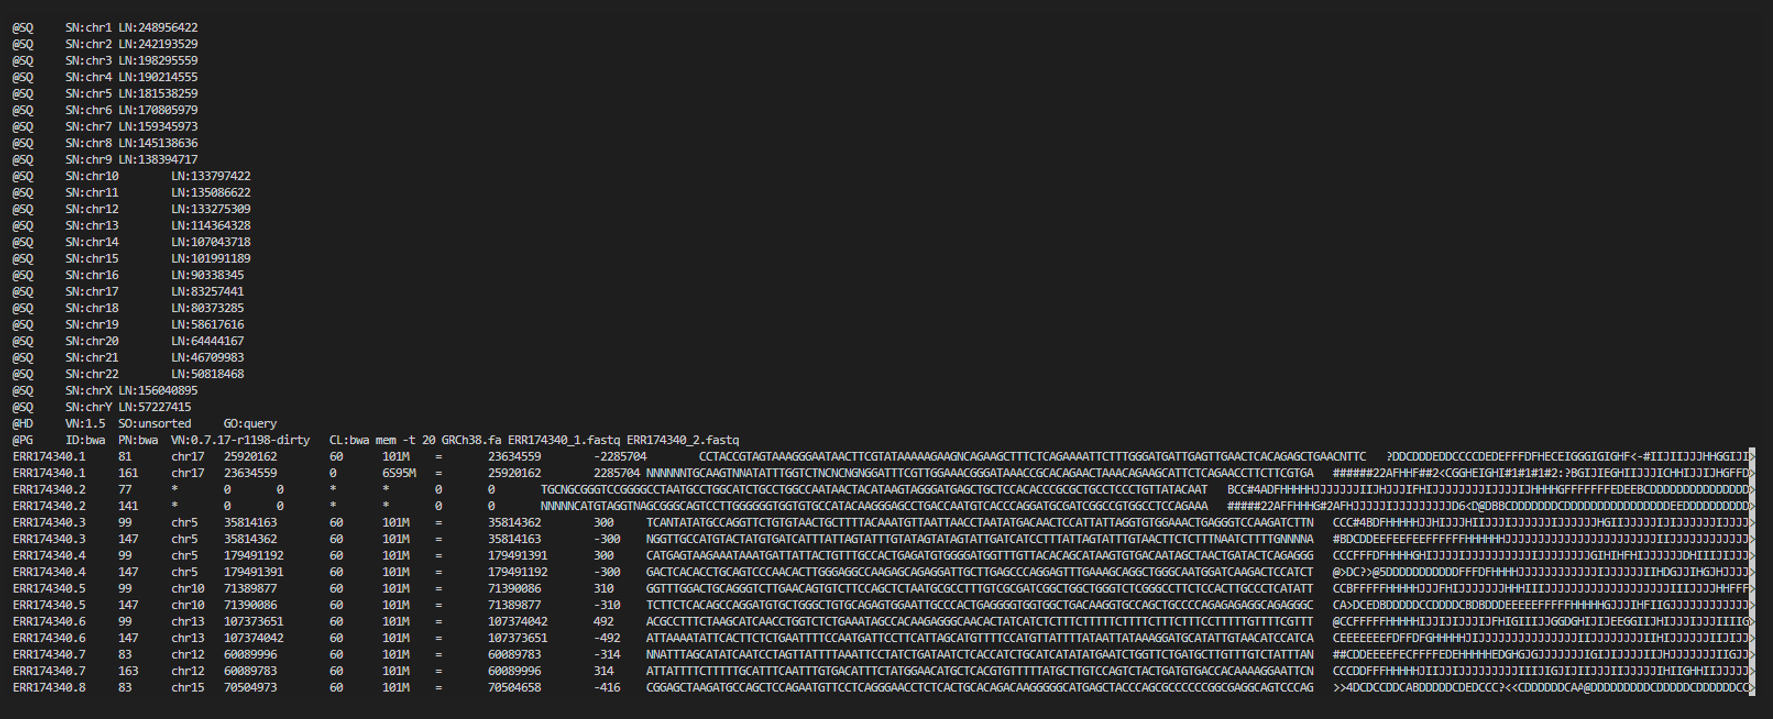
\includegraphics[scale=0.3]{figures/Example_for_SAM_file.png}
	\caption{Example for SAM format.}
	\label{fig:SAM format} % \ref{this label}
\end{figure}

The SAM file is a file stored in SAM format, while Binary Alignment Map file (BAM file) is a binary file corresponding to a SAM file, which stores the same data in a compressed binary representation. The BAM file is a compact and indexable representation of nucleotide sequence alignments, which can effectively compress the storage space and quickly query specific locations.

\subsection{Variant Call Format}
Variant Call Format (VCF) specifies the format of the text file used in bioinformatics for storing gene sequence variants~\cite{Danecek2011VCF}. A VCF file is a file stored in VCF, which consists of two parts, the header and the VCF body. As shown in Figure \ref{fig:VCF format}, the header is the beginning of the file and provides the metadata describing the body of the file; the header starts with "\#" and the special keyword is indicated by \#\#.

\begin{figure}[h!]
	\centering
	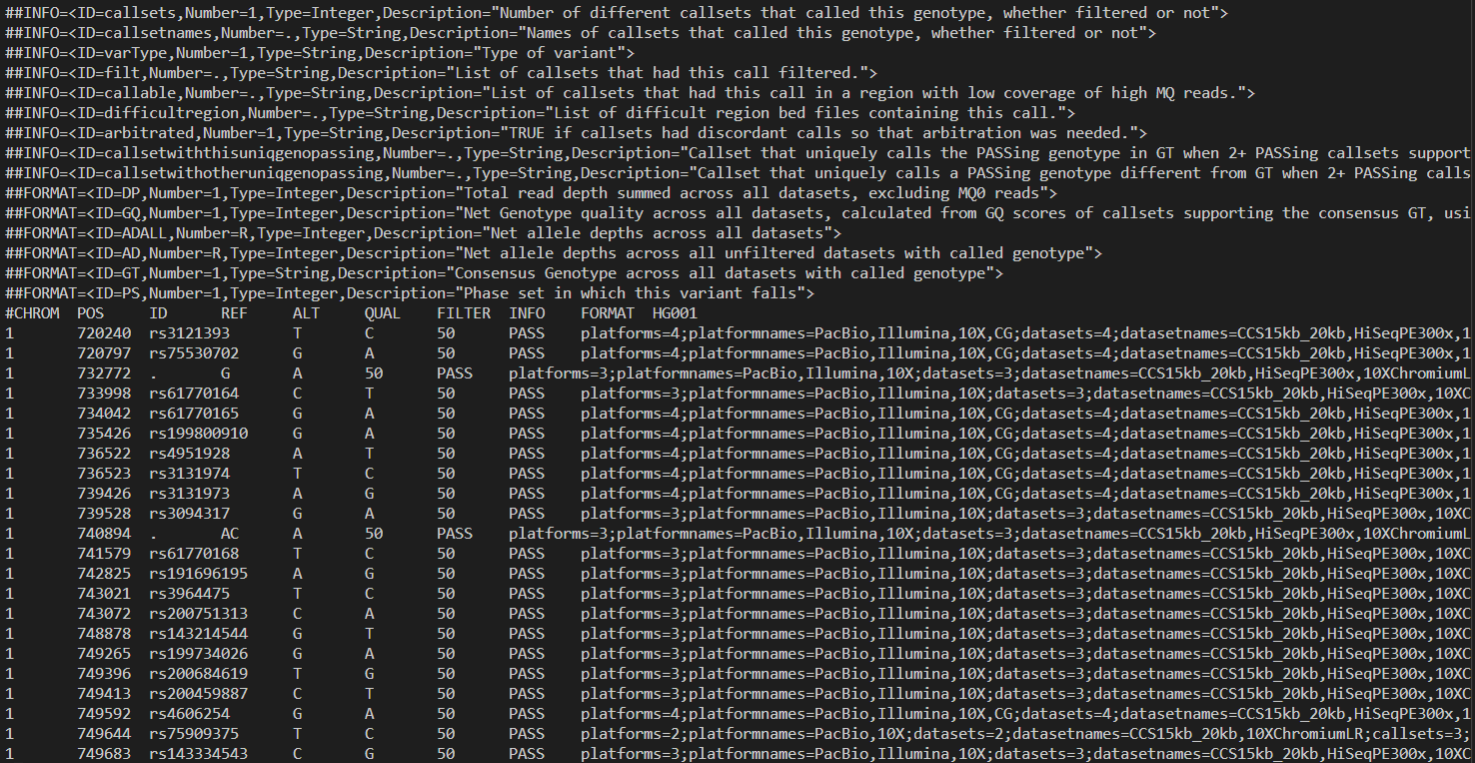
\includegraphics[scale=0.3]{figures/Example_for_VCF_file.png}
	\caption{Example for VCF format.}
	\label{fig:VCF format} % \ref{this label}
\end{figure}

\subsection{FASTQ and FASTA format}
The FASTA format is a text-based format for representing nucleotide sequences or amino acid (protein) sequences, where nucleotides or amino acids are represented as single-letter codes~\cite{Lipman1985FASTA}. The format originated from the FASTA software package and has now become a very common standard in the field of bioinformatics. In the FASTA file(Figure \ref{fig:FASTA format}), each sequence is stored with a ">" in the first line, followed by a summary description of the sequence, and then by the sequence information.

\begin{figure}[h!]
	\centering
	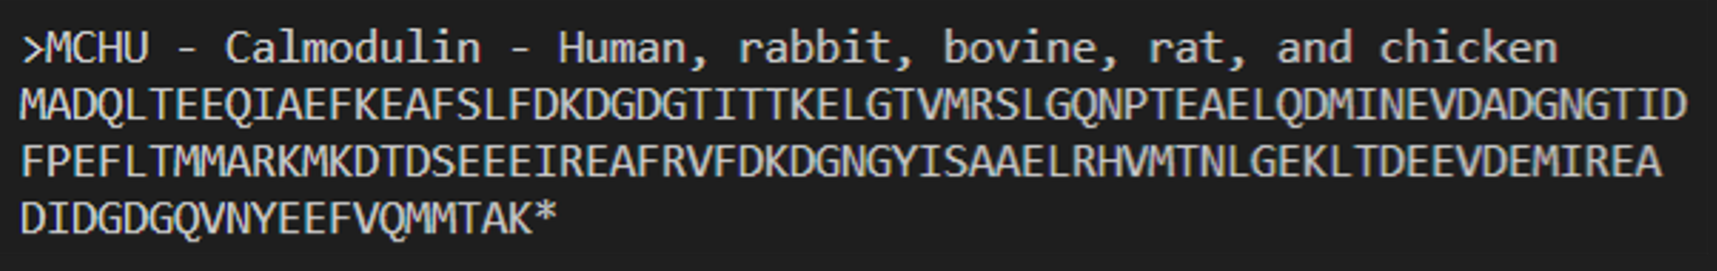
\includegraphics[scale=0.4]{figures/Example_for_FASTA_format.png}
	\caption{Example for FASTA format.}
	\label{fig:FASTA format} % \ref{this label}
\end{figure}

The FASTQ format is a text-based format for storing information about biological sequences and their quality scores, where both the sequence and the quality scores are represented by a single ASCII character~\cite{Cock2010FASTQ}. Since it combines the sequence and the associated quality score of each base, FASTQ has become a common file format for sequencing read data.

\begin{figure}[h!]
	\centering
	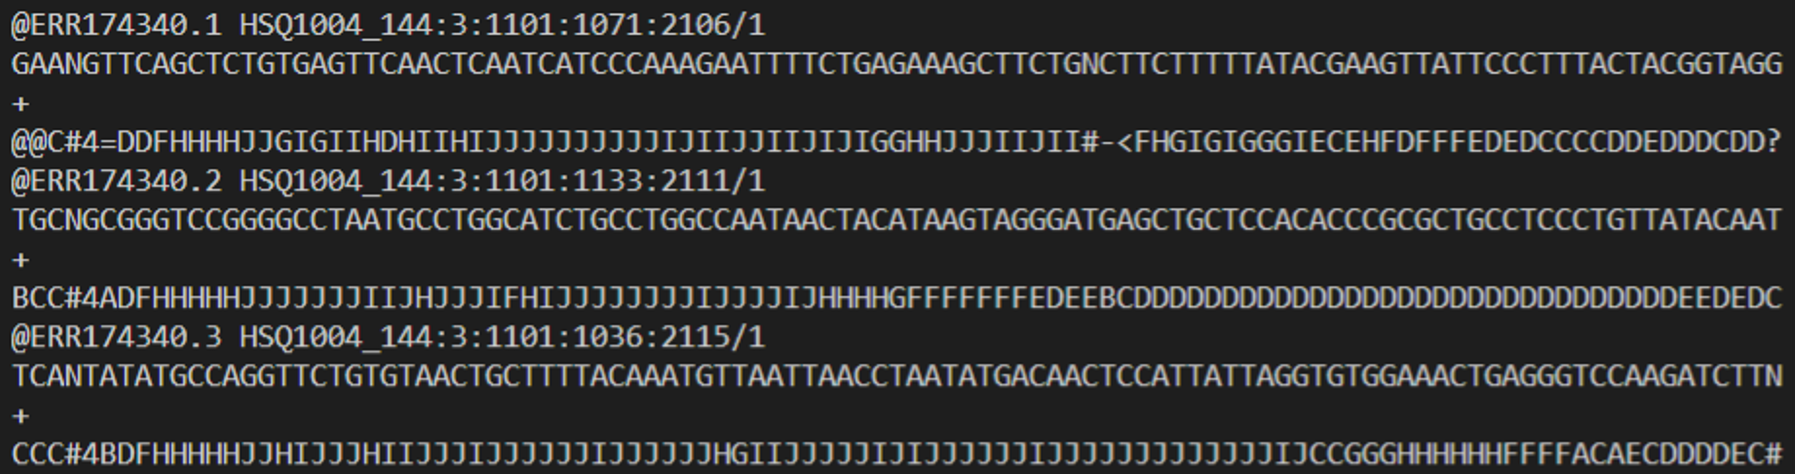
\includegraphics[scale=0.3]{figures/Example_for_FASTQ_format.png}
	\caption{Example for FASTQ format.}
	\label{fig:FASTQ format} % \ref{this label}
\end{figure}

In the FASTQ file(Figure \ref{fig:FASTQ format}), a sequence usually consists of four lines. The first line starts with "@", followed by the identifier of the sequence and the description information. The second line is the sequence information, consisting of A, T, C, G, N, etc. The third line starts with a "+", after which the sequence identifier and description information can be added again. The fourth line is the quality score information, which corresponds to the sequence in the second line, and must be the same length as the second line.

\section{EAGLE}
This section introduces the function and concept of EAGLE, a variant calling evaluator based on an explicit probability model, which was previously studied.

As shown in Figure \ref{fig:EAGLE workflow}, the main function of EAGLE is to take the three files provided by the user as input:the reference genome in FASTA format file, the called variants in a variant call format file(VCF file) and the aligned sequencing reads in a Binary Alignment Map file(BAM file). Then return the likelihood score of each candidate variants.

\begin{figure}[h!]
	\centering
	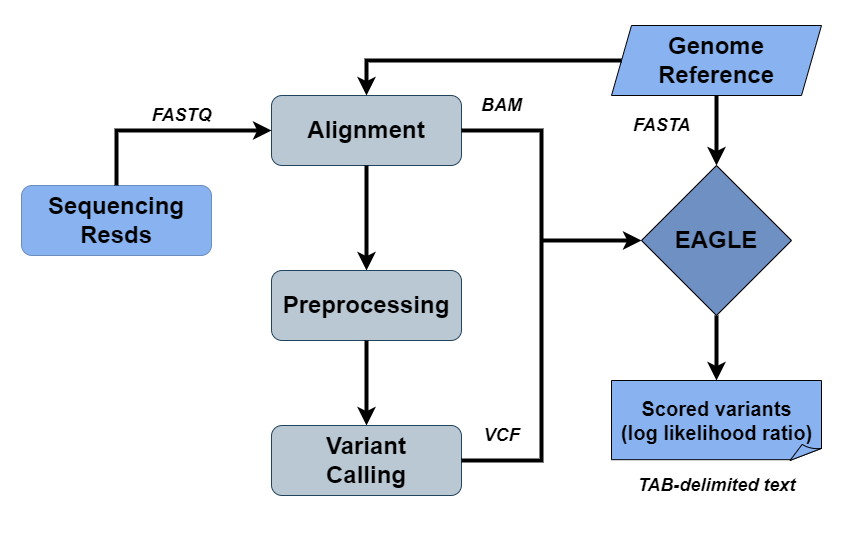
\includegraphics[scale=0.3]{figures/EAGLE.png}
	\caption{A high level overview of the EAGLE workflow. (Figure reproduced from Kuo et al.~\cite{Kuo2018EAGLE})}
	\label{fig:EAGLE workflow} % \ref{this label}
\end{figure}

The main concept is that, during variant calling, various uncertainties such as sequencing errors, inaccurate alignments and low read coverage can cause errors, which can affect downstream analysis. Therefore, EAGLE includes candidate variants in the explicit hypothesis of individual genomes, and then calculates the odds of the sequencing reads under each hypothesis. To explicitly assess the degree of match between given individual sequencing data and the list of candidate variants, and then to deal with these possible errors and uncertainties.

In conclusion, the more uncertain the quality of the data, the less credible the analysis will be. Therefore, in principle, the likelihood score calculated by EAGLE can be used to rank the reliability of putative variants and enhance the credibility of downstream analysis.

\section{Reference Bias}
Sequencing data analysis often begins with aligning reads to a reference genome. Conventionally, read alignment is performed using a linear reference genome.Because the linear reference genome contains only a single sequence, it does not capture the genomic diversity of a population. Because of the difference between the reference genome and the individual being sequenced, alignment tools map reads to the wrong location or fail to match the occurrence(Figure \ref{fig:Reference bias}). This problem can lead to false negative or false positive variant calls.

There have been many studies discussing how to mitigate the impact of reference bias, such as genome graph aligners, or using high-coverage NGS data, to improve the reference genome to include the diversity of the human genome~\cite{Günther2019Refbias, Chen2021Refbias}.

\begin{figure}[h!]
	\centering
	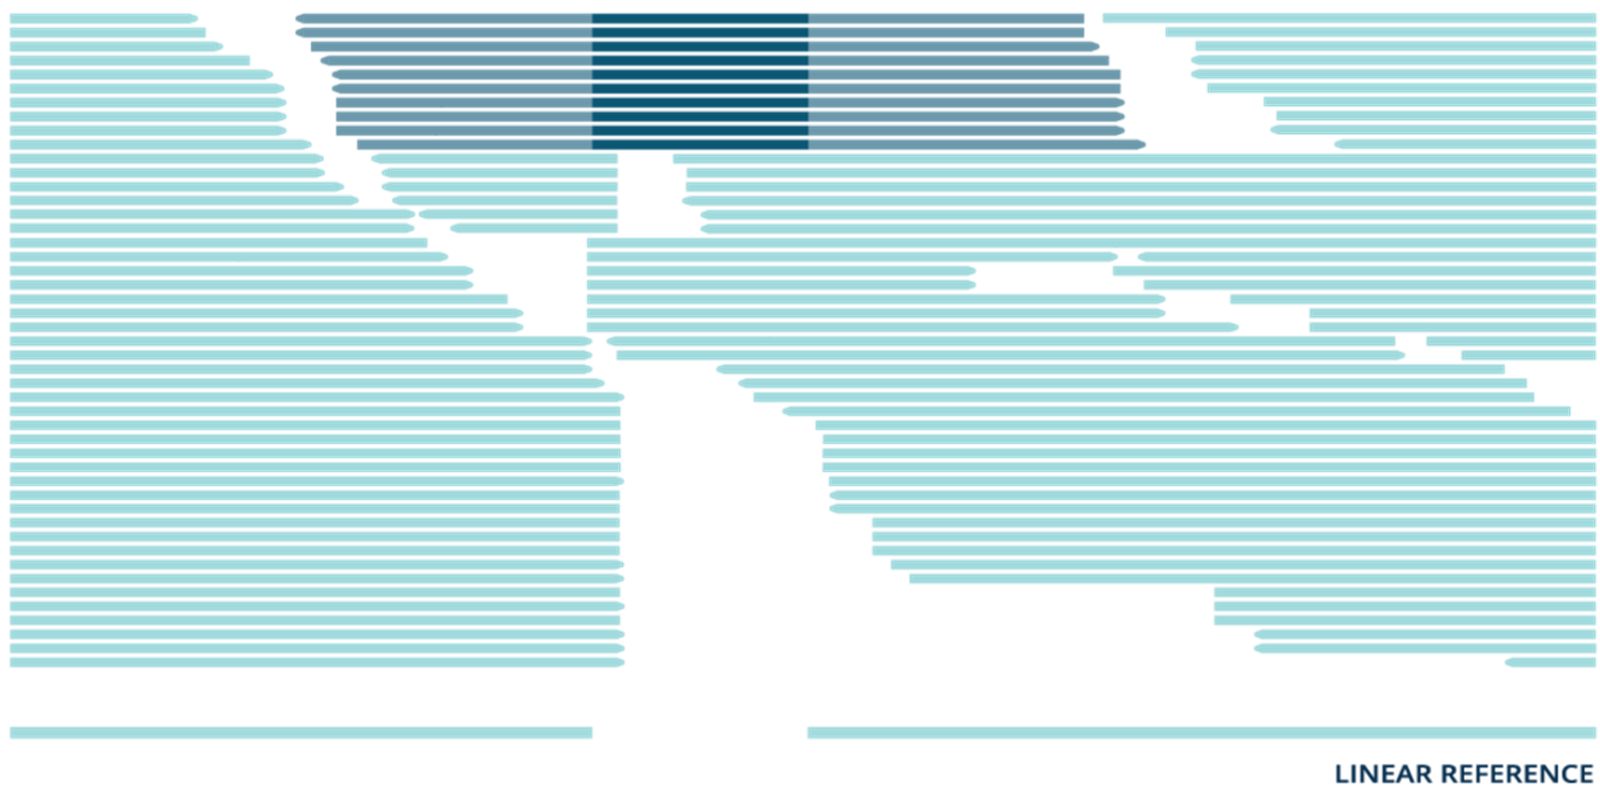
\includegraphics[scale=0.25]{figures/Reference_bias.png}
	\caption{Reference bias. Only a small portion of the read containing inserts (dark blue) are mapped to the correct positions during the alignment to the reference genome~\cite{Lau2017Refbias}.}
	\label{fig:Reference bias} % \ref{this label}
\end{figure}

\section{Hypothetical Sequence}
\begin{figure}[h!]
	\centering
	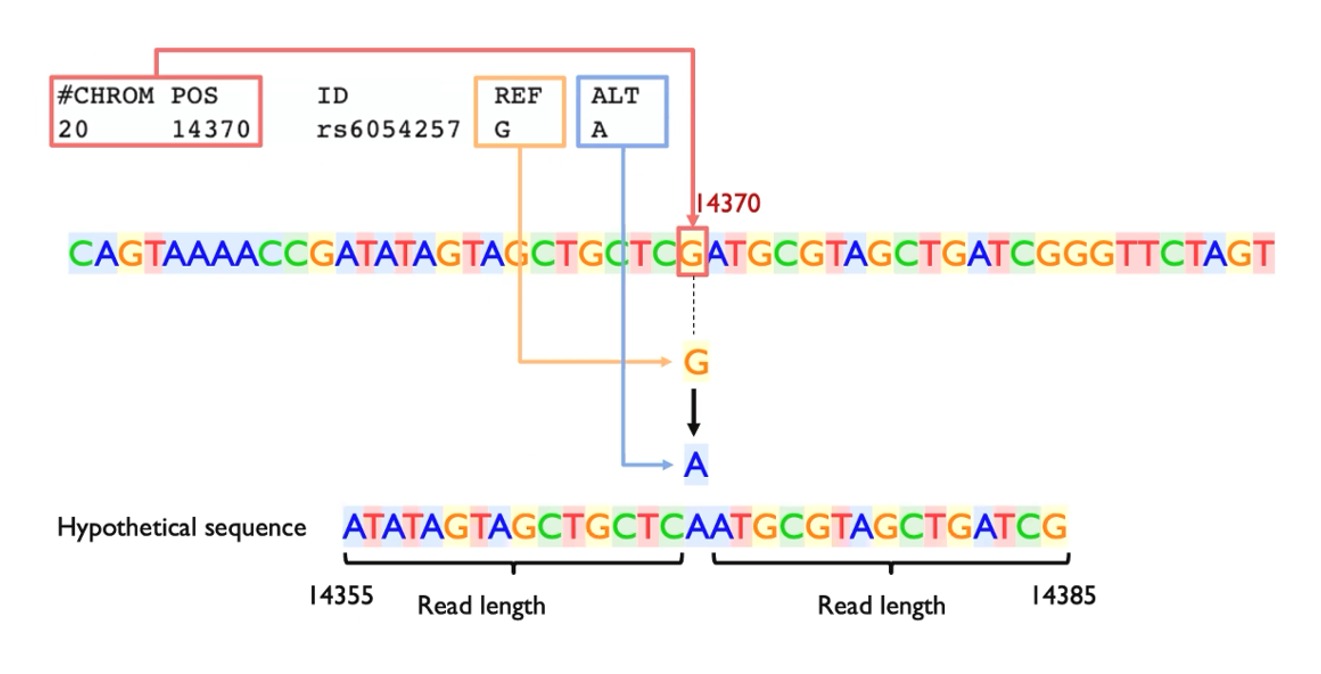
\includegraphics[scale=0.25]{figures/Hypothetical_Sequence.png}
	\caption{A Hypothetical Sequence constructed from single nucleotide polymorphisms. (Figure reproduced from Su.~\cite{Su2021RI})}
	\label{fig:Hypothetical Sequence} % \ref{this label}
\end{figure}
In our previous study, the reference genome was modified to construct the Hypothetical Sequence to reduce the effect of reference bias.

We construct a Hypothetical Sequence by replacing the pre-variant sequence with the after-variant sequence according to the variant position, and retrieve the part of the reference genome before and after the position with a read length.

Since we simulate the occurrence of mutations in the reference sequence by combining the variant to generate Hypothetical Sequence, the reference genome captures the genomic diversity of the entire population and find the reads that match our Hypothetical Sequence in the FASTQ file to reduce the impact of the reference bias.
\section{read-index}
If we search for reads matching our Hypothetical Sequence in FASTQ file by traditional method, we need to compare all the reads with Hypothetical Sequence. In our case, for each variant, we will create a Hypothetical Sequence to search for matching reads, which will take a lot of our time.

Therefore, in our previous study, we investigated the variation of overall time complexity when indexing the Hypothetical Sequence and reads respectively in order to improve the search efficiency. Finally, we decided to index the reads to generate the read-index, which helps us to find the read matching Hypothetical Sequence quickly.
\\
\begin{figure}[h!]
	\centering
	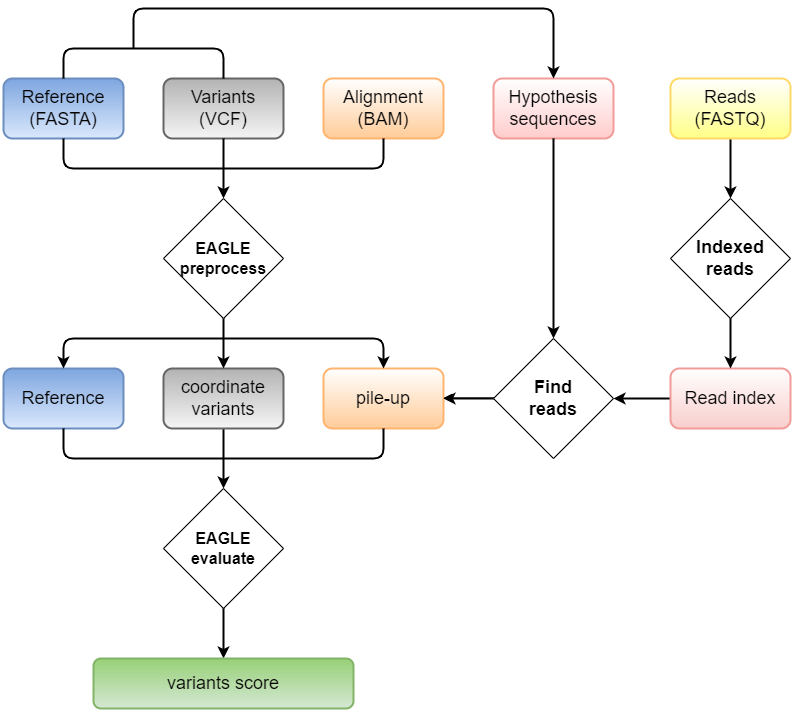
\includegraphics[scale=0.7]{figures/afterEAGLE.png}
	\caption{The core workflow of EAGLE after adding read-index to reduce reference bias.}
	\label{fig:EAGLE with read-index} % \ref{this label}
\end{figure}

\chapter{Related Works}
This chapter will briefly introduce the variant callers to be used in this study, first introducing GATK HaplotypeCaller~\cite{Poplin2018GH}, then BCFtools~\cite{Danecek2021BCFtools}, and finally Platypus~\cite{Rimmer2014Platypus}. Each variant caller will input a BAM file for variant calling, and output a VCF file as the result.
\section{GATK HaplotypeCaller}
GATK HaplotypeCaller is able to call SNPs and indels by performing local de novo assembly on haplotypes of active regions. In other words, whenever it encounters a region that is likely to be mutated, GATK HaplotypeCaller discards the existing mapping information and completely reassembles the read of the region. This allows GATK HaplotypeCaller to be more accurate when calling regions that were previously difficult to call, for example, when they contain different types of variants very close to each other. This also allows GATK HaplotypeCaller to perform better than location-based callers in calling indels.

The following is the workflow of GATK HaplotypeCaller(Figure \ref{fig:GATK HaplotypeCaller}):\\
1. Identify active regions based on variation evidence (mapping information) and determine which regions the program needs to operate on.\\
2. For each active region, the program builds a De Bruijn-like graph to reassemble active regions and determine which haplotypes are likely to be present in the data. The Smith-Waterman algorithm is then used to reassemble each haplotype with the reference haplotype to identify the potential variation sites.\\
3. Calculate the likelihoods of the haplotypes based on the given read data. i.e. for each active region, the program uses the PairHMM algorithm to align each read and each haplotype to obtain the allele likelihoods for each potential variant site.\\
4. For each potential variant site, the program applies Bayes' rule and calculates the likelihood of each genotype for each sample using the likelihood of the allele for the given read data, and then assigns the most likely outcome to that sample.

\begin{figure}[h!]
	\centering
	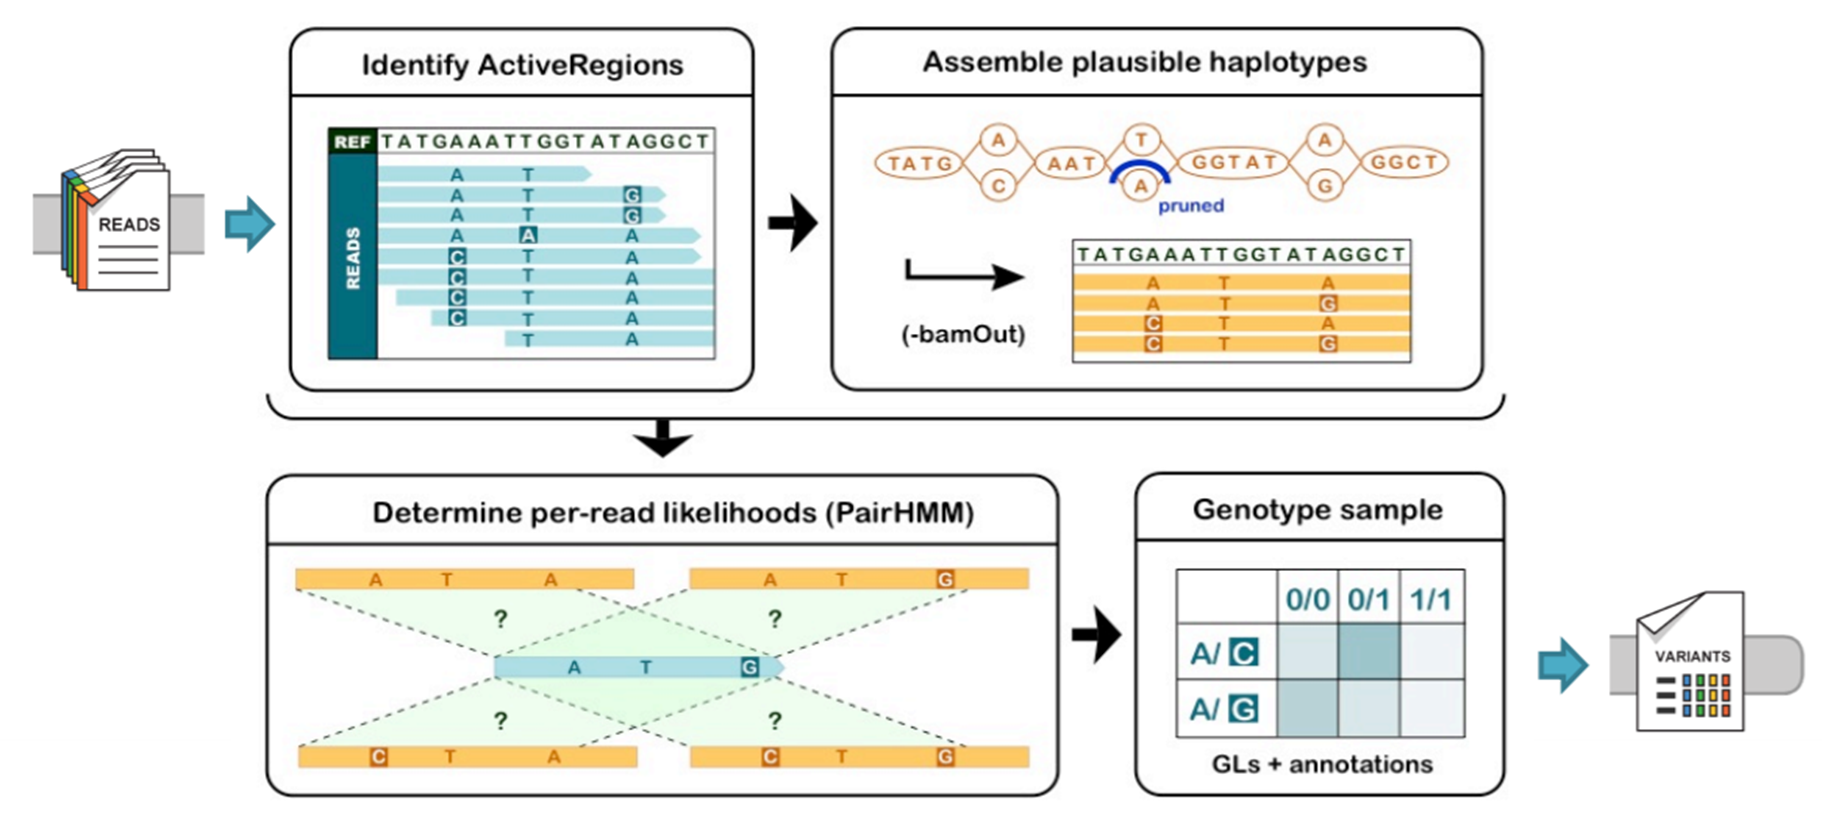
\includegraphics[scale=0.25]{figures/GATK_HaplotypeCaller.png}
	\caption{The workflow of GATK HaplotypeCaller. (Figure reproduced from Poplin, Ryan, et al.~\cite{Poplin2018GH})}
	\label{fig:GATK HaplotypeCaller} % \ref{this label}
\end{figure}

\section{BCFtools}
BCFtools generates candidate variant directly from the results of independent mapping of each read to the reference genome, and simulates sequencing errors and variant calling by using Bayesian inference~\cite{Li2011SAMtools, Li2010SAMtools}.

BCFtools performs variant calling in two steps. The first "mpileup" part generates genotype likelihoods at each genomic position with coverage. The second "call" part makes the actual calls.

In previous versions, BCFtools was usually combined with SAMtools' mpileup command for variant calling. Since both SAMtools and BCFtools are updated very quickly, if you install the wrong version of the tool, it will easily cause errors. Therefore, in order to reduce the problems caused by inappropriate versions, the BCFtools development team added the mpileup feature to BCFtools.

\section{Platypus}
As shown in Figure \ref{fig:Platypus}, Platypus generates candidate variants by using local de novo assembly followed by local rearrangement and probabilistic haplotype estimation~\cite{Rimmer2014Platypus}.

\begin{figure}[h!]
	\centering
	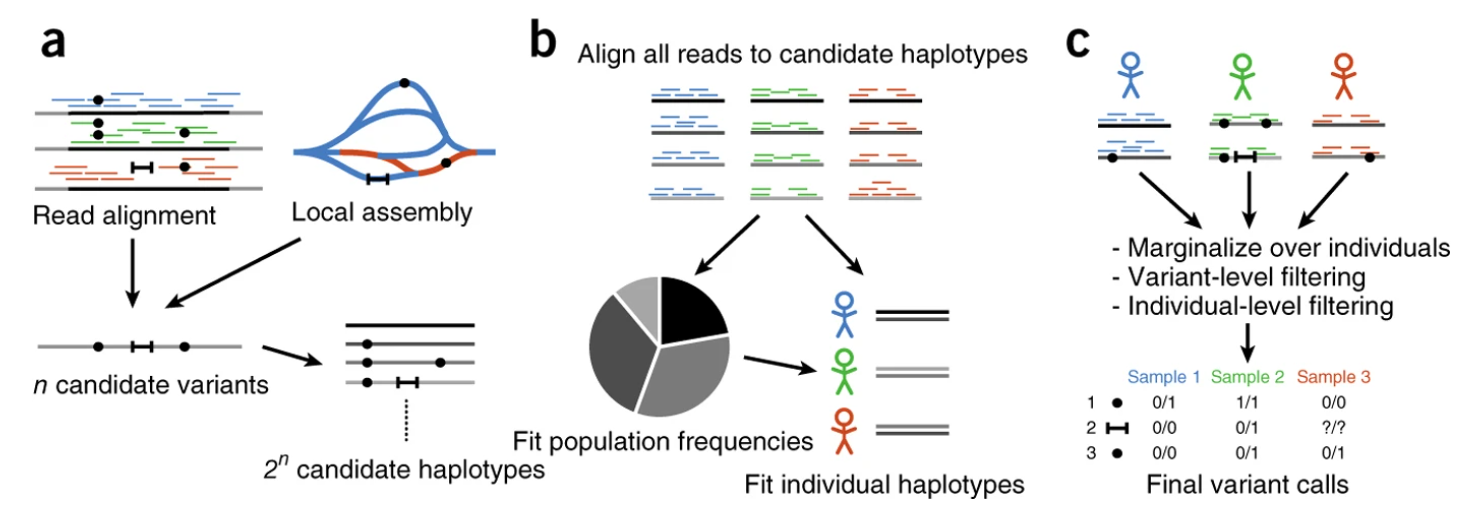
\includegraphics[scale=0.4]{figures/Platypus.png}
	\caption{The pipeline of the Platypus algorithm contains three stages. (Figure reproduced from Poplin, Rimmer, Andy, et al.~\cite{Poplin2018GH})}
	\label{fig:Platypus} % \ref{this label}
\end{figure}

First, Platypus generates a set of candidate variants according to the algorithm. Three sources of candidate variants can be considered: variants directly supported by the read alignment, variants identified by the assembly, and variants from external sources. For n variants, this results in $2^{n}$ haplotypes (disregarding excluded combinations due to overlap).

Then, the likelihood of haplotype was calculated, that is, given the probability of the haplotype read: $p(r|h)$, where r and h denote read and haplotype, respectively. After calculating $p(r|h)$ for all combinations of reads and haplotypes, the Expectation-Maximization (EM) algorithm was used to estimate the probability of each haplotype under the diploid genotype model.

\begin{equation}
  L(R|\{ {h_i,f_i} \}) = \prod_{\text{sample} \hspace{0.5mm} s}\sum_{\text{haplotypes} \hspace{0.75mm} i,j} {f_if_j} \prod_{\text{reads} \hspace{0.5mm} r \in R_s} (\frac{1}{2}p(r|h_i) + \frac{1}{2} p(r|h_j))
\end{equation}

Here, $f_i$ denotes the frequency of \hspace{0.05mm} haplotype $h_i$ in the population; $a$ is the number of alleles considered, $R$ and $R_s$ denote the set of all reads, and reads from sample $s$ respectively, and the sum over haplotypes extends over all ordered pairs $(i,j)$, i.e.\ genotypes.

Finally, we break up called haplotypes into their constituent variants and calculate variant-specific genotype calls and likelihoods by marginalizing over the other variants in the region.
\begin{equation}
  P[v|R] = \frac{P(v)L(R| \{ {h_i,f_i} \} _{i=1...a})}        {P(v)L(R| \{ {h_i,f_i} \}_{i=1...a})+(1-P(v))L(R|\{ {h_i,\frac{f_i}{1-F_v} \} _{i\in I_v}})}
\end{equation}
where $P(v)$ is the prior probability of observing variant $v$. The likelihood of reads given haplotypes and their frequencies is computed as

\begin{equation}
  L(R|\{ {h_i,f_i} \}_{i=1...a}) = \prod_{sample \hspace{0.5mm} s}\sum_{haplotypes \hspace{0.75mm} i,j} {f_if_j} \prod_{reads \hspace{0.5mm} r \in R_s} (\frac{1}{2}p(r|h_i) + \frac{1}{2} p(r|h_j))
\end{equation}

\chapter{Experimental Workflow}
\section{Dataset}
In this study, in order to test the performance of the new version of EAGLE on real sequencing data, we use an exome sequencing dataset (Garvan HG001) from Genome-In-A-Bottle (GIAB)~\cite{Zook2014GIAB} and a 200× whole genome sequencing dataset from Illumina Platinum Genomes (IPG) to NA12878 (cell line of an individual from a CEPH pedigree) real data were tested~\cite{Eberle2021IPG}.

\begin{table}[h!]
	\centering
	\scalebox{1.2}{
	\begin{tabular}{|c|c|c|}
		\hline
		\diagbox[innerwidth=2cm]{Use}{From} & GIAB & IPG\\
		\hline
		Reference & GRCh37 & GRCh38\\
		\hline
		Read & Exome Data & 200xWGS Data\\
		\hline
		System & HiSeq2500 & HiSeq2000\\
		\hline
	\end{tabular}}
	\caption{The Dataset of Experiment.}
	\label{table:1}
\end{table}

The benchmark from IPG is a high confidence callset constructed using variant callers such as FreeBayes, Platypus, and GATK to construct the GRCh38 human gene reference sequence(Figure \ref{fig:IPG VariantCaller}).
The benchmark from GIAB is a high confidence callset for the GRCh37 human genome reference sequence using FreeBayes, SAMtools, and GATK.

Since the performance was evaluated using the above data in the previous study, we would like to use the same dataset to present and discuss the results in this study.But the benchmarks were constructed from variant calls made by the same tools we are comparing against, there may be some bias in the following results.

\begin{figure}[h!]
	\centering
	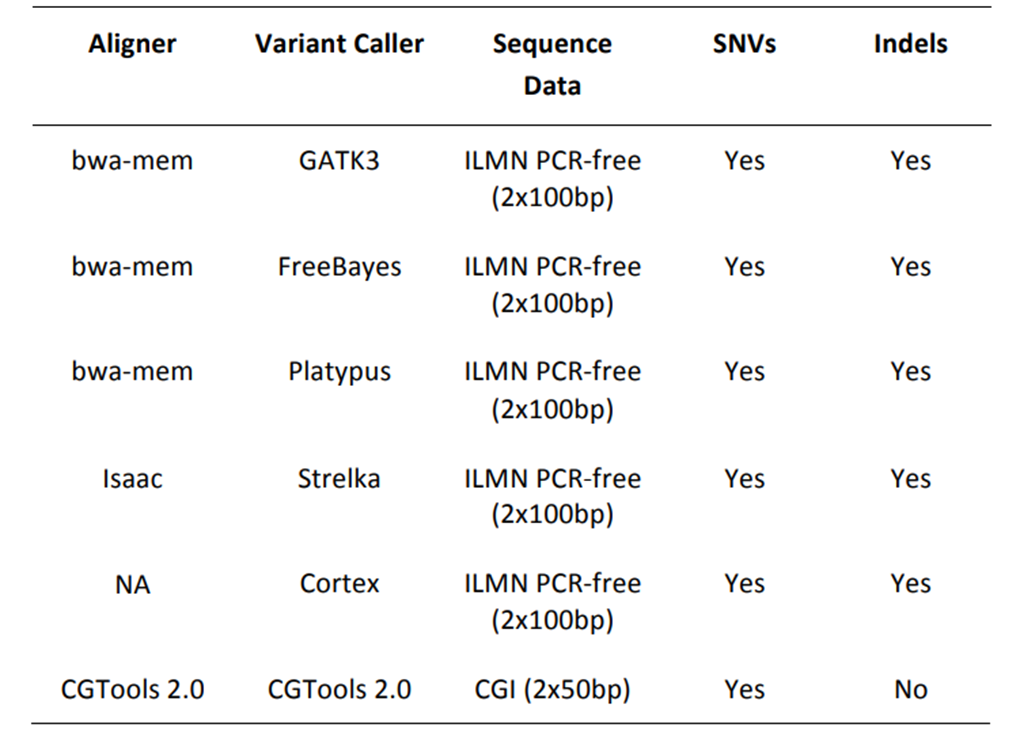
\includegraphics[scale=0.4]{figures/IPG_VariantCaller.png}
	\caption{The IPG sequence data and variant calling pipelines. (Figure reproduced from Eberle, MA et al.~\cite{Eberle2021IPG})}
	\label{fig:IPG VariantCaller} % \ref{this label}
\end{figure}

\section{Data Preprocessing}
In the previous section we introduced two sets of datasets to be used, in this section we will briefly describe the flow of data preprocessing.\\
First, we refer to the GATK 'best practices' preprocessing steps to practice our process~\cite{Geraldine2013GATKBestP}, the process of constructing a BAM file is as follows:\\
1. Create an index of the reference genome for subsequent usage.\\
2. Use BWA-MEM to perform Read mapping~\cite{Li2013BWA}.\\3. Convert the obtained SAM file to BAM file to save storage space.\\
4. Sort the BAM file from the smallest to the largest according to the chromosome name and coordinate order.\\
5. Do Label read groups with Picard AddOrReplaceReadGroups on BAM file~\cite{AddOrReplaceReadGroups}.\\
6. For BAM file use Picard MarkDuplicates identifies duplicate reads and remove it~\cite{MarkDuplicates}.

In the second step, we use the generated BAM format alignment data to make call variants using the variant caller introduced in Chapter 3.

Finally, we canonicalize the complex variants using \texttt{vt normalize} for each variant callset we obtained~\cite{Tan2015Vt}.

\section{Plotting PR Curves}
According to the EAGLE mentioned in Subsection 2.2, we will input the variant callset obtained in Subsection 4.2 in the format of a vcf file. This is used to obtain the marginal posterior probabilities for each candidate variants.
Since the variant evaluator EAGLE evaluates the confidence level of the variants in the input file, we want to focus on the correct determination of the positive samples.
However, even if the number of negative samples in the data set is much larger than the number of positive samples, the Precision-Recall Curves (PR Curve) is still a valid reference indicator.
Therefore, we rank the marginal posterior probabilities of the obtained results and the quality scores of each variant caller separately. Finally, a PR Curve was obtained to evaluate the performance of our new version of EAGLE.

\chapter{Results and Discussion}
\section{Experimental Results}
In this section, the dataset and data preprocessing process introduced in the previous section will be applied to plot the PR Curve to present the changes between the new version of EAGLE and the previous version. Due to the large amount of biological data, the variation data of chromosome 22 will be extracted for the presentation of the results in this study.

In addition to showing the performance of Insertion and Deletion (indel) and Single Nucleotide Polymorphism (SNP) separately (Figure \ref{fig:The result of IPG dataset}(a,c) and Figure \ref{fig:The result of IPG dataset}(b,d)), we have also plotted two comparative graphs to facilitate the discussion.
The first one is to plot EAGLE with read-index and the three variant callers using marginal posterior probabilities and quality scores (Figure \ref{fig:The result of IPG dataset}(a,b)).
The second one is to plot the best performing curves of EAGLE, EAGLE with read-index and variant caller (Figure \ref{fig:The result of IPG dataset}(c,d)).

\begin{figure}[h!]
	\centering
	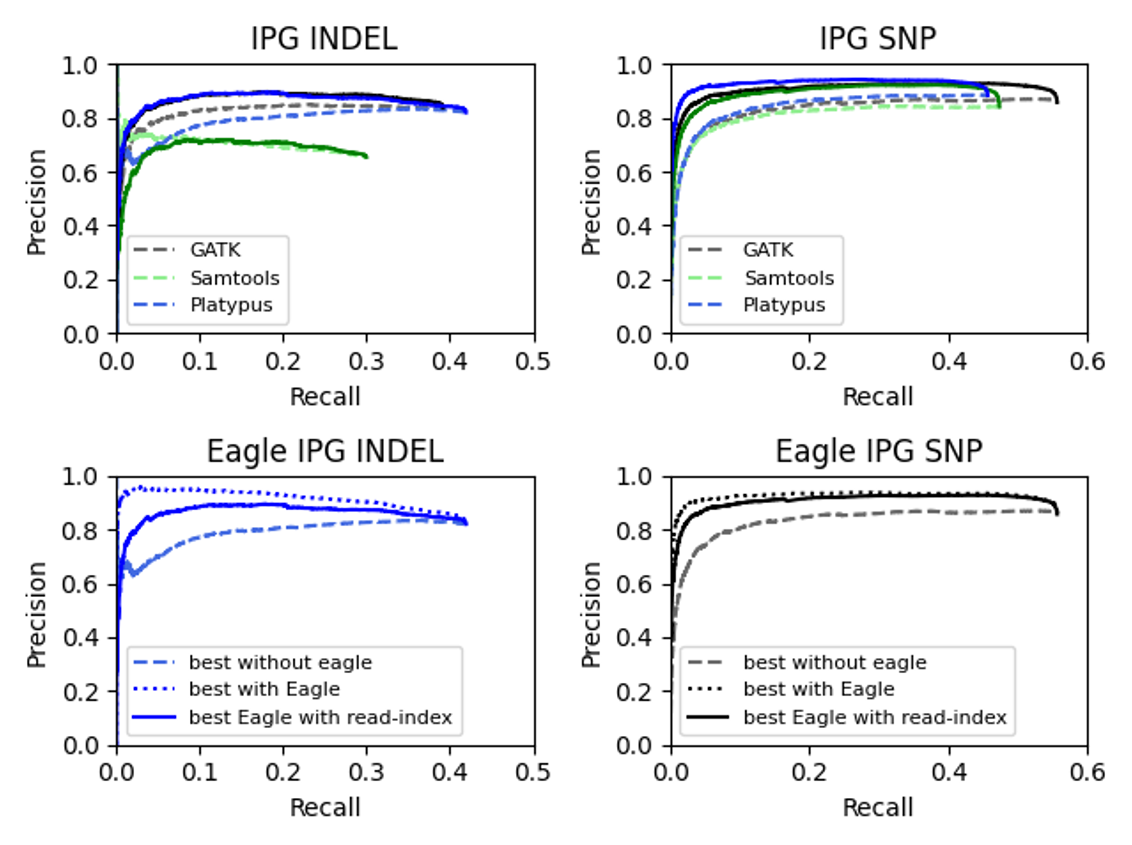
\includegraphics[scale=0.45]{figures/IPG_result.png}
	\caption{Precision and recall for NA12878 for whole genome sequencing data in Illumina Platinum Genome benchmark.}
	\label{fig:The result of IPG dataset}
\end{figure}

\begin{figure}[h!]
	\centering
	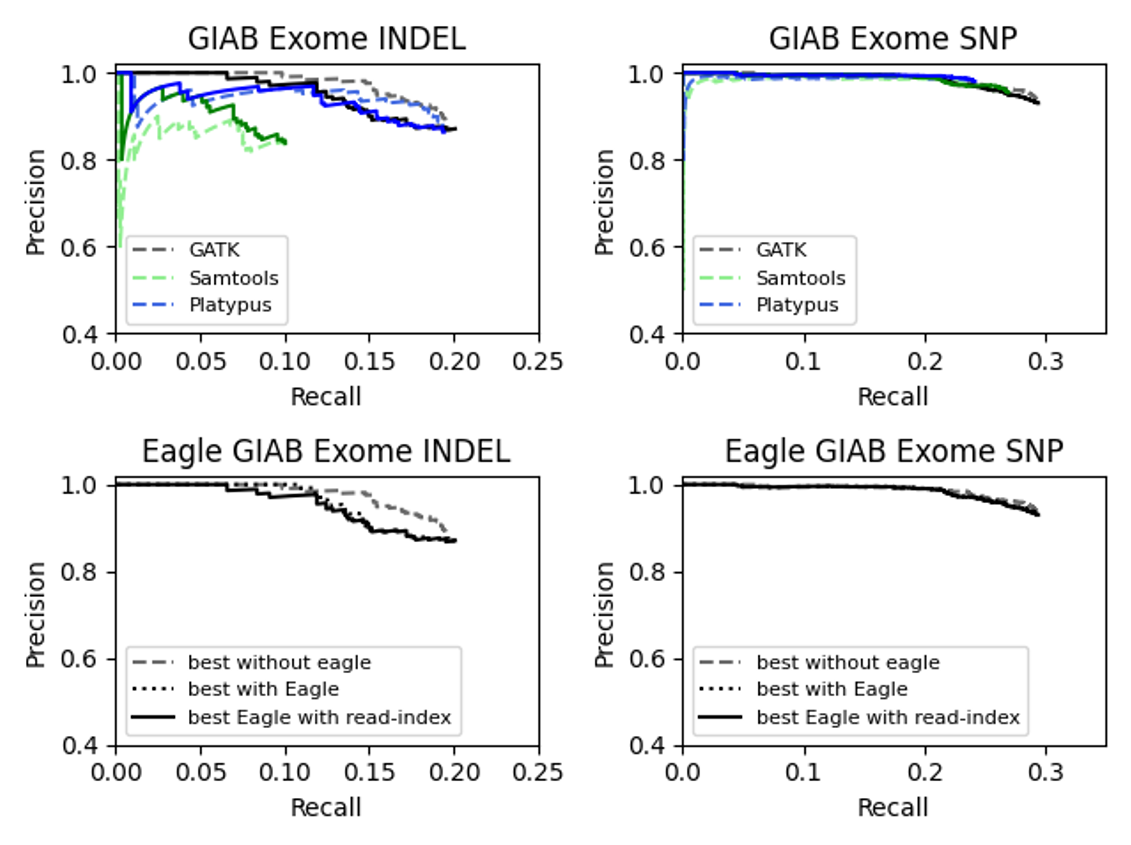
\includegraphics[scale=0.45]{figures/GIAB_result.png}
	\caption{Precision and recall for the NA12878 Genome-In-A-Bottle benchmark.}
	\label{fig:The result of GIAB dataset}
\end{figure}

For the above results, we can notice that the new version of EAGLE has a significantly higher precision than the variant caller in ranking putative variants on whole genome sequencing data(Figure \ref{fig:The result of IPG dataset}). However, contrary to the expectation, compared with the previous version of EAGLE, there was a decrease in precision at the same recall level in both indel and SNP.  There was no significant change in the exome sequencing data.

\begin{figure}[h!]
	\centering
	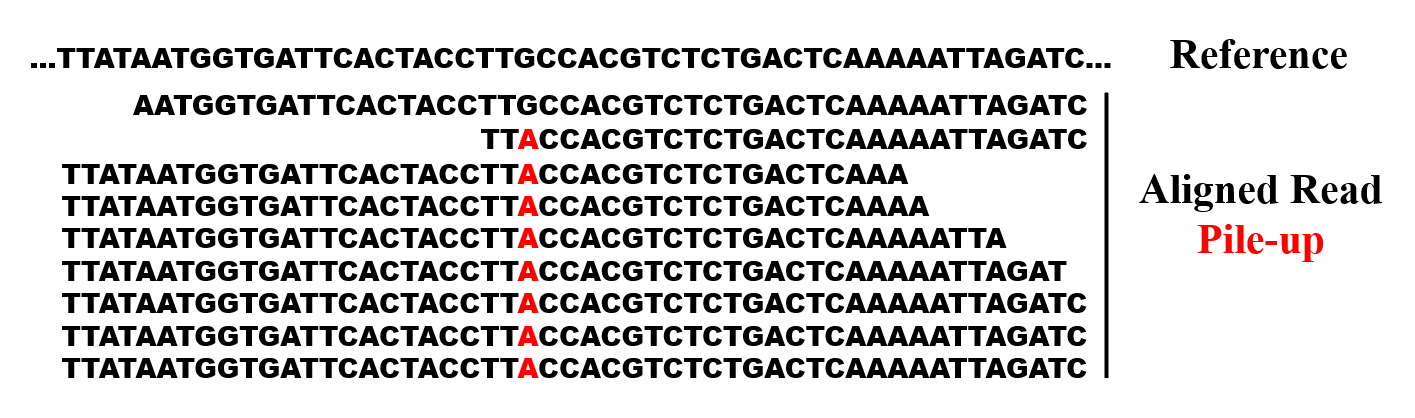
\includegraphics[scale=0.3]{figures/Pileup.png}
	\caption{Example for pile-up.}
	\label{fig:Example for pile-up}
\end{figure}

\section{Checking the pile-up}
As mentioned above, we got the opposite result than expected in the new version of EAGLE.  Therefore, in order to find the reason for the problem, we examined the pile-up before and after using read-index, expecting to get an explanation for the lower-than-expected results.

We ranked EAGLE with read-index (EAGLE-WRI) with the marginal posterior probabilities calculated by EAGLE and found that EAGLE-WRI increased the variant with lower probability in EAGLE very much. Therefore, we wanted to check the top variants with higher probability in EAGLE-WRI, which did not appear in the benchmark. So we check this variant in the case that no new reads are added to the pile-up.

As shown in Table \ref{table:2}, we manually checked 30 indel and 25 SNP cases respectively. Among the 30 cases of indel, we found that 21 cases with high probability were not found in the benchmark data, but after checking the original BAM file, we found that 13 of them showed support for the possibility of variation. Among the 25 cases of SNP, we found that 17 examples with higher probability were not found in the benchmark data, but after checking the original BAM file, we found that 12 of them showed support for the possibility of variation. In the following, we will show 3 indel cases(Figure \ref{fig:The Example of pile-up for indel1}, \ref{fig:The Example of pile-up for indel2}, \ref{fig:The Example of pile-up for indel3}) and 3 SNP cases respectively(Figure \ref{fig:The Example of pile-up for SNP1}, \ref{fig:The Example of pile-up for SNP2}, \ref{fig:The Example of pile-up for SNP3}).

As mentioned in subsection 1.1, because there are many uncertainties in variant calling, such as sequencing error, inaccurate alignment, and low read coverage. Therefore, we believe that the degradation of performance may be related to the absence of some variant in the benchmark.

\begin{table}[h!]
	\centering
	\scalebox{0.8}{
	\begin{tabular}{|c|c|c|c|c|c|}
		\hline
		\multicolumn{2}{|c|}{\multirow{2}*{\diagbox[innerwidth=2cm]{Type}{State}}}  & \multicolumn{2}{c|}{Before checking} & \multicolumn{2}{c|}{After manual checking}\\
		\cline{3-6}
		\multicolumn{2}{|c|}{} & In Benchmark & Not in Benchmark & Benchmark or Plausible mutations & Appears wrong\\
		\hline
		\multicolumn{2}{|c|}{indel} & 9 & 21 & 22 & 8 \\
		\hline
		\multicolumn{2}{|c|}{SNP} & 8 & 17 & 20 & 5 \\
		\hline
	\end{tabular}}
	\caption{Checking the pile-up for mutations}
	\label{table:2}
\end{table}

\begin{figure}[h!]
	\centering
	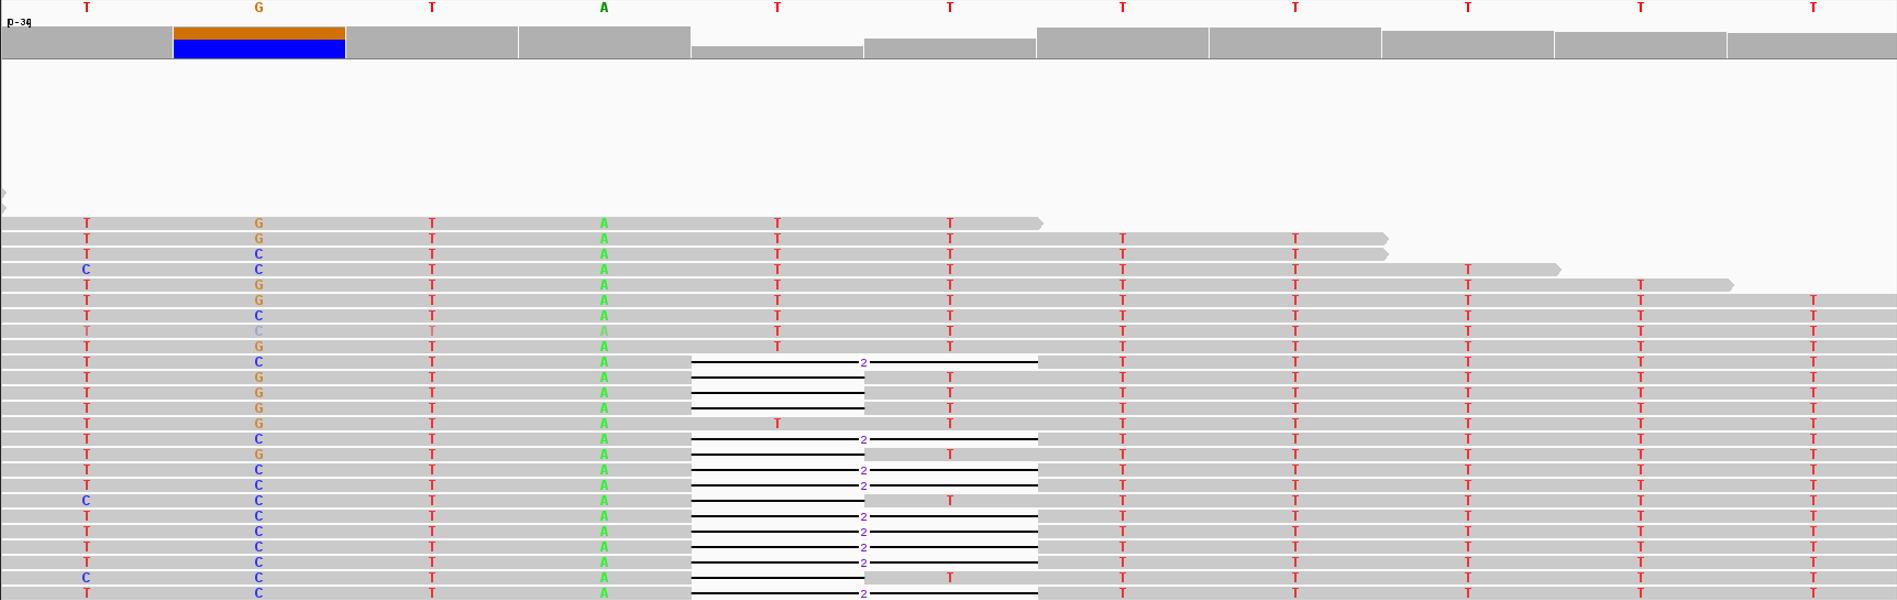
\includegraphics[scale=0.3]{figures/INDEL1.png}
	\caption{The Example1 of pile-up for indel.}
	\label{fig:The Example of pile-up for indel1} 
\end{figure}

\begin{figure}[h!]
	\centering
	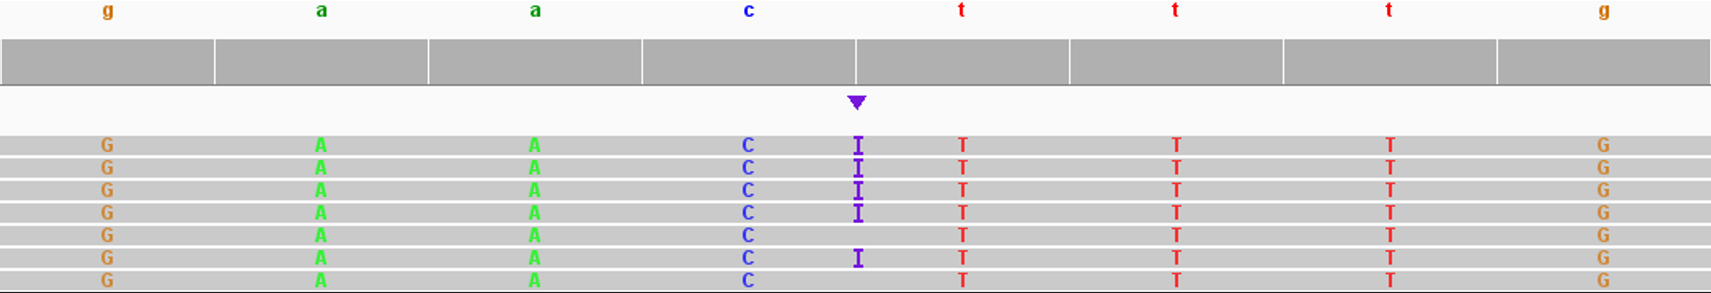
\includegraphics[scale=0.3]{figures/INDEL2.png}
	\caption{The Example2 of pile-up for indel.}
	\label{fig:The Example of pile-up for indel2} % \ref{this label}
\end{figure}

\begin{figure}[h!]
	\centering
	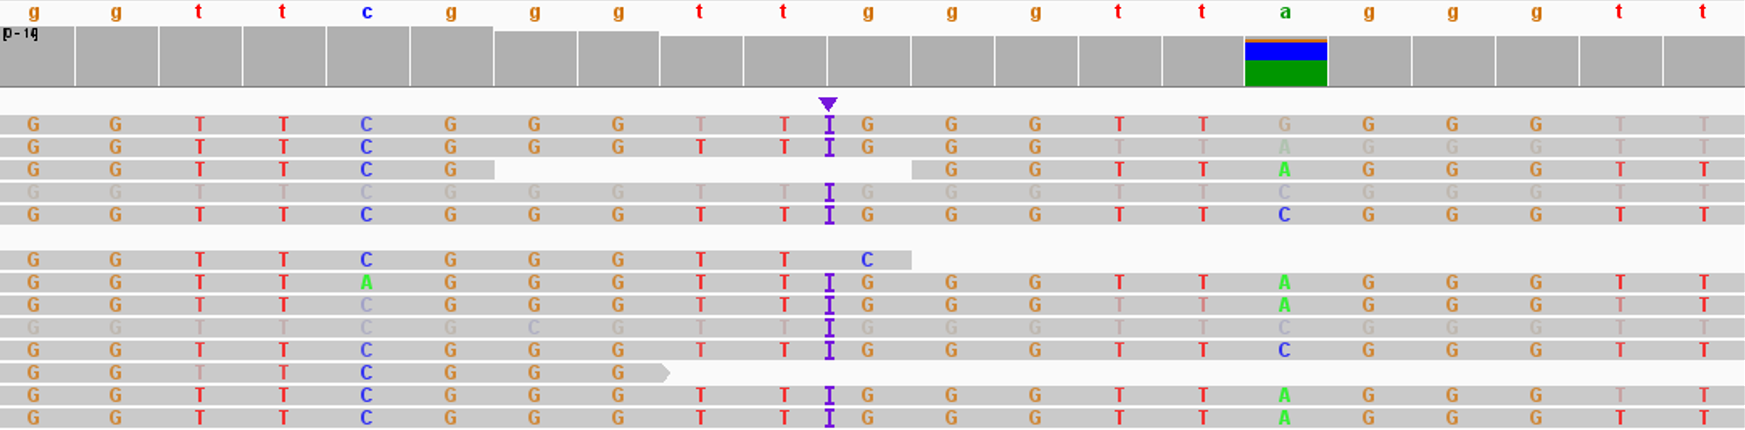
\includegraphics[scale=0.3]{figures/INDEL3.png}
	\caption{The Example3 of pile-up for indel.}
	\label{fig:The Example of pile-up for indel3} % \ref{this label}
\end{figure}

\begin{figure}[h!]
	\centering
	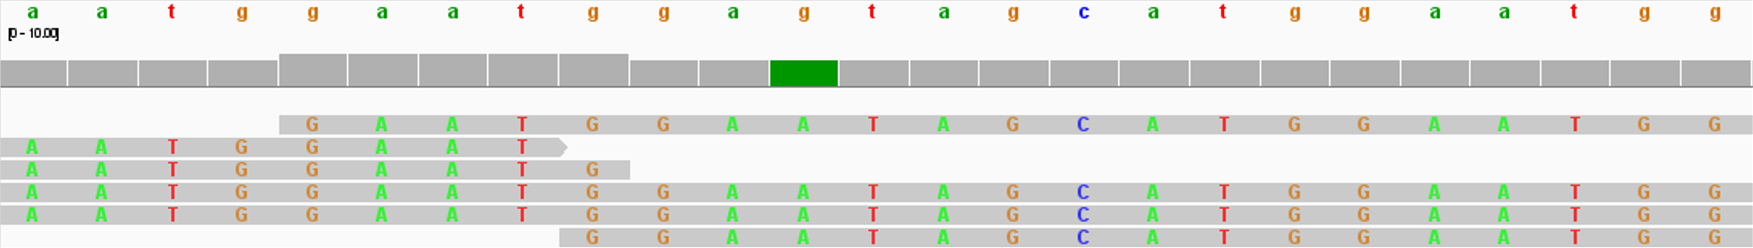
\includegraphics[scale=0.3]{figures/SNP3.png}
	\caption{The Example1 of pile-up for SNP.}
	\label{fig:The Example of pile-up for SNP1} % \ref{this label}
\end{figure}

\begin{figure}[h!]
	\centering
	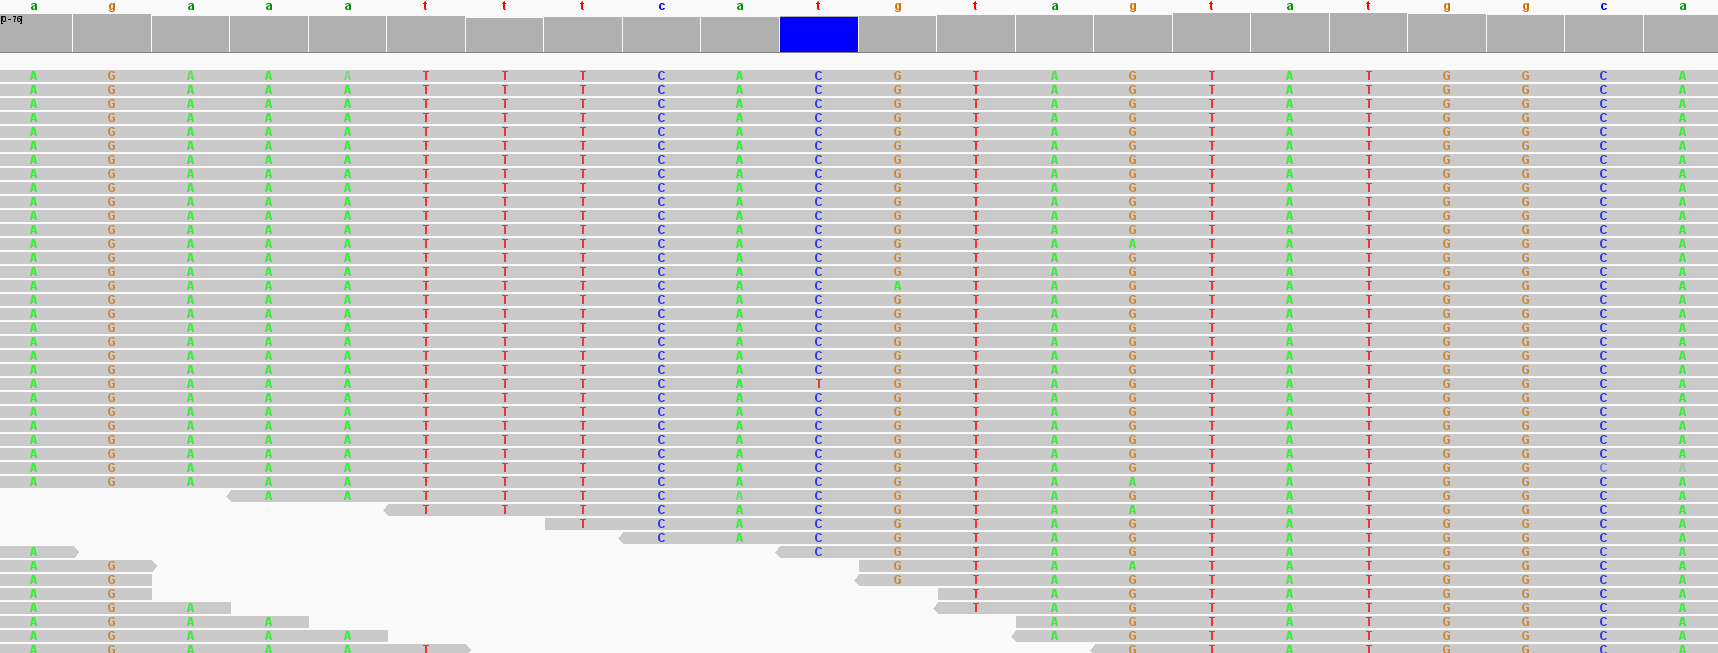
\includegraphics[scale=0.25]{figures/SNP2.png}
	\caption{The Example2 of pile-up for SNP.}
	\label{fig:The Example of pile-up for SNP2} % \ref{this label}
\end{figure}

\begin{figure}[h!]
	\centering
	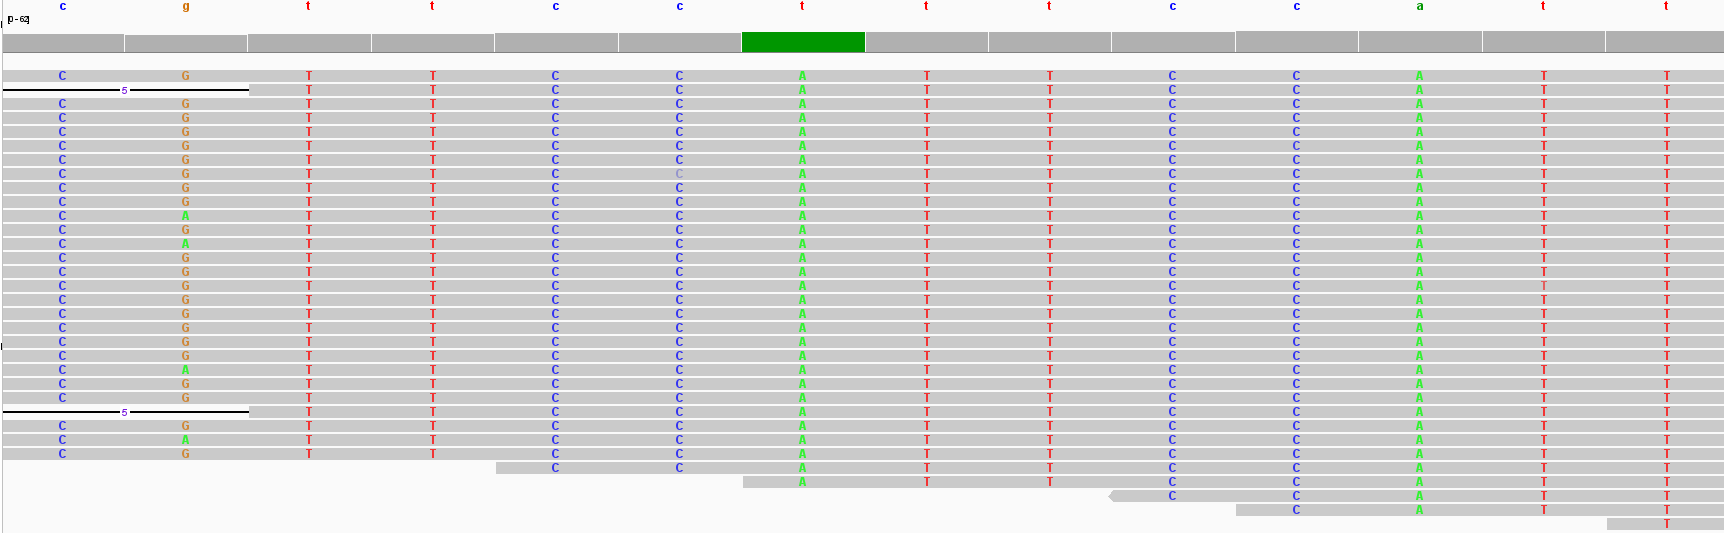
\includegraphics[scale=0.25]{figures/SNP1.png}
	\caption{The Example3 of pile-up for SNP.}
	\label{fig:The Example of pile-up for SNP3} % \ref{this label}
\end{figure}


\section{Multi-mapping detection}
In the results showcase, we found that the benchmark data may have some missing variation. In the above process, it is also shown that EAGLE-WRI supports more variants not found in the benchmark than before. In other words, EAGLE-WRI adds many reads to the pile-up as described in subsection 2.4.

However, since there are many similar regions in the human genome reference sequence, it is possible that the reads added to this region are from reads that have been mapped to other positions in the reference genome. To rule out the possibility of such a problem, we will perform a check. We extracted the high probability examples from EAGLE-WRI to examine the problem. 

The results showed that among the 30 examples of SNPs and indel, we found 2 and 1 variant with multi-mapping phenomenon respectively. Therefore, in the examination of this problem, we can probably exclude the possibility of evaluation errors in EAGLE-WRI due to multi-mapping.

\begin{figure}[h!]
	\centering
	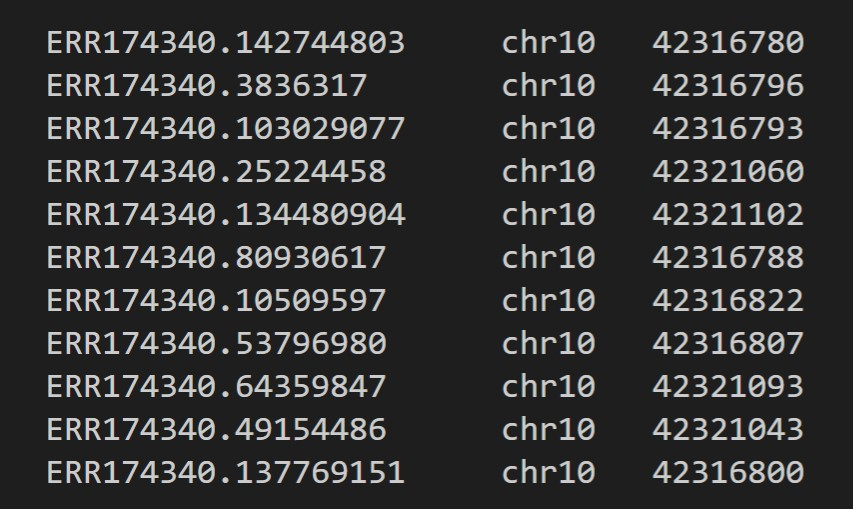
\includegraphics[scale=0.4]{figures/chr10mulltimapping.jpg}
	\caption{The example of SNP with multimapping phenomenon.}
	\label{fig:The example of SNP with multimapping phenomenon} % \ref{this label}
\end{figure}

\begin{figure}[h!]
	\centering
	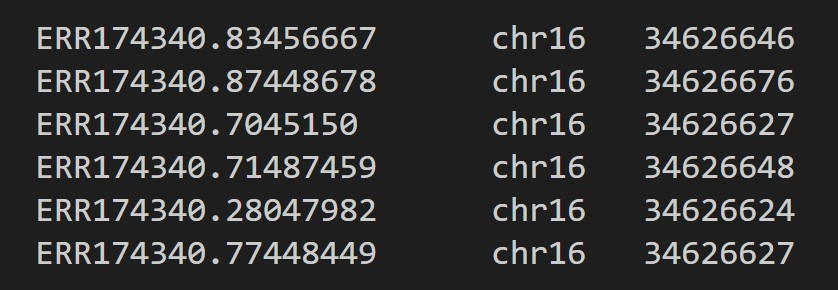
\includegraphics[scale=0.4]{figures/indelmulltimapping.jpg}
	\caption{The example of indel with multimapping phenomenon.}
	\label{fig:The example of indel with multimapping phenomenon} % \ref{this label}
\end{figure}

\chapter{Conclusion and Future Work}
\section{Conclusion}
In our previous study, we extended the functionality of EAGLE to reduce the effect of reference bias and to improve the accuracy of EAGLE in assessing variation. We have also demonstrated in previous simulations that the modified EAGLE is effective in eliminating the effects of reference bias, but we have not yet verified the accuracy of EAGLE on real data.

However, when we evaluated EAGLE by precision versus recall, we found a significant decrease in precision at the same recall level in the whole genome sequencing data. Therefore, in our subsequent study, we examined several cases that led to the decrease in performance and found that the decrease in performance might be related to the missing variant in the benchmark data. However, the missing variants could not be ruled out because the benchmark used more stringent conditions to call variant.

We also detect the areas where EAGLE gives a higher chance of variation. This is to avoid that EAGLE highly supports variants that are not found in the benchmark because of adding too many similar regions of reads to pile-up. The results show that only a very small number of the examples we examined had the Multi-mapping case. Therefore, we can generally rule out the possibility of evaluation errors in EAGLE.

As mentioned above, in this study, we speculate that the decrease in performance may be due to a variation in the missing part of the benchmark data. As a result of the above examination, we generally exclude the possibility of evaluation errors in the new version of EAGLE. Therefore, it can be shown that EAGLE has the ability to detect missing benchmark data. However, more significantly, we only examined a small number of cases during the study, so we cannot be completely sure of our findings. As a result, we need to examine all cases of performance degradation more rigorously in future studies to support our findings and to examine whether there are systemic defects in the new version of EAGLE.
\section{Future Work}
In this paper, we examined both the pile-up and the multi-mapping detection manually. This consumes a lot of our time and limits our ability to make a more comprehensive evaluation of the results. As future work, we should implement an automatic process to achieve both of these tests, as well as a rigorous follow-up examination of performance using GIAB exome sequencing data, which may also reveal the same problems. This will give a more complete evaluation of EAGLE with read-index and make it more useful for NGS data analysis.

\newpage
\AddToContents{Bibliography}
\printbibliography


\end{document}
